\def\mySecNum{5.3}
\mySection{\mySecNum~Forward contracts on stock}
%-------------- start slide -------------------------------%{{{ 1
\begin{frame}[fragile,t]
\begin{center}
	\textcolor{magenta}{\bf Forward price} is the future value of the \textcolor{cyan}{prepaid forward price}:

	\begin{align*}
		F_{0,T} = \text{FV}\left(F_{0,T}^p\right)
	\end{align*}

	\vfill

	\begin{minipage}{0.5\textwidth}
		\begin{myexample}
				Continuous dividends
				\begin{align*}
					F_{0,T} = S_0 e^{(r-\delta)T}
				\end{align*}
				\begin{itemize}
					\item $r$: risk-free rate.
					\item $\delta$: the dividend yield.
				\end{itemize}
		\end{myexample}
	\end{minipage}
\end{center}
\end{frame}
%-------------- end slide -------------------------------%}}}
%-------------- start slide -------------------------------%{{{ 1
\begin{frame}[fragile,t]
\begin{align*}
	\text{\textcolor{magenta}{Forward premium}} = \frac{F_{0,T}}{S_0}
\end{align*}
\bigskip
\begin{align*}
	\text{Annualized forward premium}	 = \frac{1}{T} \ln \left(\frac{F_{0,T}}{S_0}\right)
\end{align*}
\end{frame}
%-------------- end slide -------------------------------%}}}
%-------------- start slide -------------------------------%{{{ 1
\begin{frame}[fragile,t]
	\frametitle{Does the forward price predict the future spot price?}

	\begin{center}
		Buying a stock\\
		\bigskip

		\renewcommand{\arraystretch}{1.2}
		\begin{tabular}{|c|c|c|}
			\hline
			Compensation for        & Earn                              & Buying a stock \\ \hline
			time value of the money & interest                          & \cmark         \\
			the risk of the stock   & \textcolor{magenta}{risk premium} & \cmark         \\ \hline
		\end{tabular}

		\vfill
		\mySeparateLine
		\vfill

		Entering a forward contract \\
		\bigskip

		\renewcommand{\arraystretch}{1.2}
		\begin{tabular}{|c|c|c|}
			\hline
			Compensation for        & Earn                              & Entering a forward contract \\ \hline
			time value of the money & interest                          & \xmark                      \\
			the risk of the stock   & \textcolor{magenta}{risk premium} & \cmark                      \\ \hline
		\end{tabular}
		\bigskip
	\end{center}
\end{frame}
%-------------- end slide -------------------------------%}}}
%-------------- start slide -------------------------------%{{{ 1
\begin{frame}[fragile,t]
\begin{center}
	The forward price is the \textcolor{magenta}{expected future spot price}, \\
	\textcolor{cyan}{discounted at the risk premium}.  \\
	\bigskip

	\begin{align*}
		F_{0,T} = e^{rT} \times \underbrace{F_{0,T}^p}_{=\E_0(S_T)e^{-\alpha T}} = \textcolor{magenta}{\E_0(S_T)}\textcolor{cyan}{e^{-(\alpha-r)T}}
	\end{align*}
\end{center}
\end{frame}
%-------------- end slide -------------------------------%}}}
%-------------- start slide -------------------------------%{{{ 1
\begin{frame}[fragile,t]
	\frametitle{Creating a synthetic forward contract}
	\begin{center}
		Assuming that the dividends are continuous and paid at the rate $\delta$. \\
		\bigskip
		\bigskip

		Recall that

		\begin{gather*}
			\text{Payoff of a long forward position at expiration} \\
			||                                                     \\
			S_T - F_{0,T}                                          \\
			||                                                     \\
			S_T - S_0 e^{(r-\delta)T}
		\end{gather*}
	\end{center}

\end{frame}
%-------------- end slide -------------------------------%}}}
%-------------- start slide -------------------------------%{{{ 1
\begin{frame}[fragile,t]
\begin{center}
	\begin{align*}
		\text{Forward} = \text{Stock} - \text{Zero-coupon bond}
	\end{align*}

	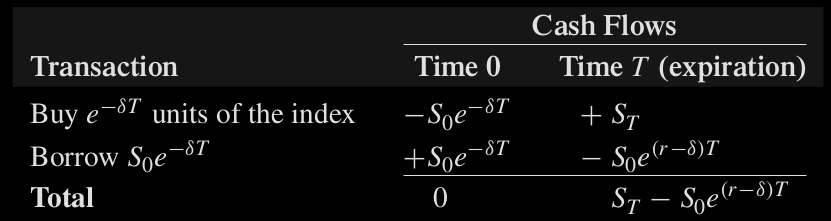
\includegraphics[scale=0.25]{figs/Table-5-3.png}
\end{center}
\end{frame}
%-------------- end slide -------------------------------%}}}
%-------------- start slide -------------------------------%{{{ 1
\begin{frame}[fragile,t]
\begin{center}
	\begin{align*}
		\text{Stock} = \text{Forward} + \text{Zero-coupon bond}
	\end{align*}

	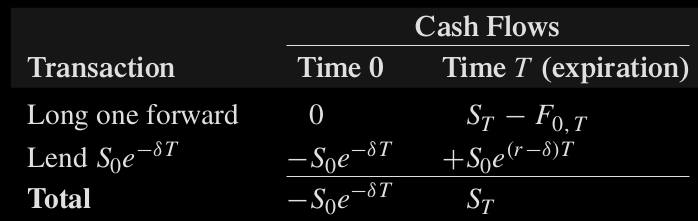
\includegraphics[scale=0.25]{figs/Table-5-4.png}
\end{center}
\end{frame}
%-------------- end slide -------------------------------%}}}
%-------------- start slide -------------------------------%{{{ 1
\begin{frame}[fragile,t]
\begin{center}
	\begin{align*}
		\text{Zero-coupon bond} =	\text{Stock} - \text{Forward}
	\end{align*}

	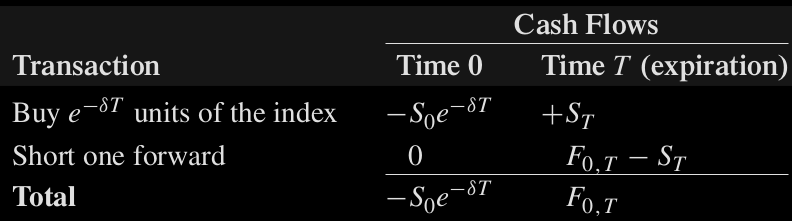
\includegraphics[scale=0.25]{figs/Table-5-5.png}
\end{center}
\end{frame}
%-------------- end slide -------------------------------%}}}
%-------------- start slide -------------------------------%{{{ 1
\begin{frame}[fragile,t]
\begin{center}
	\textcolor{magenta}{\bf Cash-and-carry} is a transaction in which one buys the underlying asset
	and short the offsetting forward contract.\\
	\bigskip


	A cash-and-carry has no risk because \\
	You have an obligation to deliver the asset\\  that you have already owned.
	\bigskip

	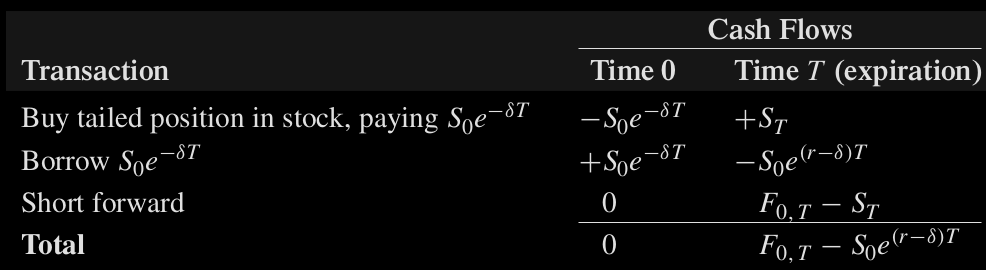
\includegraphics[scale=0.25]{figs/Table-5-6.png}

\end{center}
\end{frame}
%-------------- end slide -------------------------------%}}}
%-------------- start slide -------------------------------%{{{ 1
\begin{frame}[fragile,t]
	\begin{center}
		\textcolor{magenta}{Cash-and-carry}
		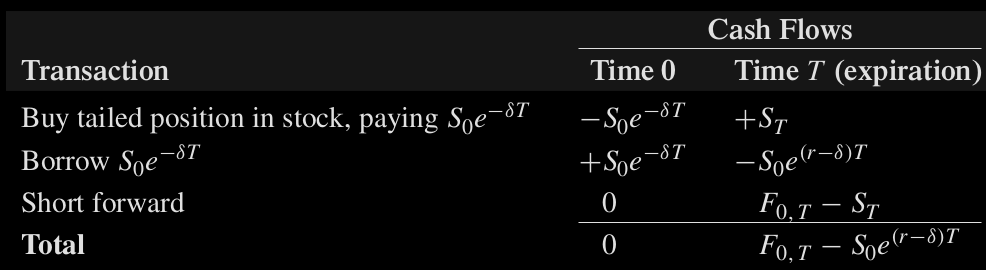
\includegraphics[scale=0.25]{figs/Table-5-6.png}

		\bigskip
		Arbitrage when $F_{0,T}\textcolor{magenta}{>}S_0 e^{(r-\delta)T}$

		\vfill
		\mySeparateLine
		\vfill

		\textcolor{cyan}{Reverse cash-and-carry}
		\bigskip

		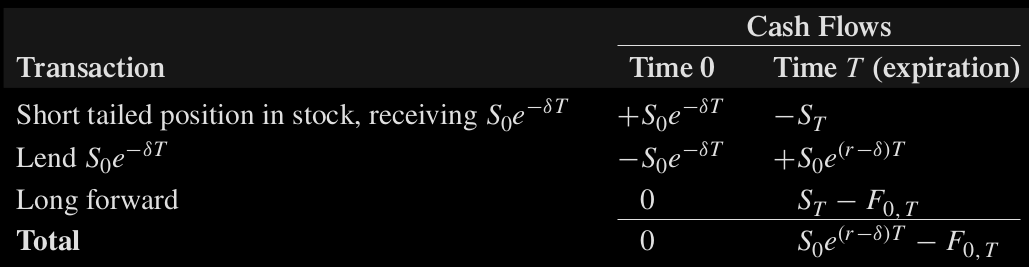
\includegraphics[scale=0.25]{figs/Table-5-7.png}
		\bigskip

		Arbitrage when $F_{0,T}\textcolor{cyan}{<}S_0 e^{(r-\delta)T}$
	\end{center}
\end{frame}
%-------------- end slide -------------------------------%}}}
